%%%%%%%%%%%%%%%%%%%%%%%%%%%%%%%%%%%%%%%%%%
% Engineering problems / LaTeX Template
%		Semester 6
%		Institut d'Optique Graduate School
%%%%%%%%%%%%%%%%%%%%%%%%%%%%%%%%%%%%%%%%%%
%	6N-IntNum-BlocTraitImage	/ Image processing
%%%%%%%%%%%%%%%%%%%%%%%%%%%%%%%%%%%%%%%%%%
%
% Created by:
%	Julien VILLEMEJANE - 16/jul/2024
% Fichier.sty modifié pour changer la police de caractère
%	
%
%%%%%%%%%%%%%%%%%%%%%%%%%%%%%%%%%%%%%%%%%%
% Professional Newsletter Template
% LaTeX Template
% Version 1.0 (09/03/14)
%
% Created by:
% Bob Kerstetter (https://www.tug.org/texshowcase/) and extensively modified by:
% Vel (vel@latextemplates.com)
% 
% This template has been downloaded from:
% http://www.LaTeXTemplates.com
%
% License:
% CC BY-NC-SA 3.0 (http://creativecommons.org/licenses/by-nc-sa/3.0/)
%
%%%%%%%%%%%%%%%%%%%%%%%%%%%%%%%%%%%%%%%%%

\documentclass[a4paper,11pt,titlepage]{article} % The default font size is 10pt; 11pt and 12pt are alternatives

%%%%%%%%%%%%%%%%%%%%%%%%%%%%%%%%%%%%%%%%%%%%%%%%%%%%%%%%%%%%%%%%%%%%%%%%%%%%%%%%%%%%%%%%%%%%%%%%%%%%%%%%%%%%%%%%%%%%%%%%%%%%%%%%%%%%%%%%%%%%%%%%%%%%%%%%%%%%%%%%%%%%%%%%%%%%%%%%%%%%%%%%%%%%%%%%%%%%%%%%%%%%%%%%%%%%%%%%%%%%%%%%%%%%%%%%%%%%%%%%%%%%%%%%%%%%
\usepackage{opto_elec_villemejane}

%%%%%%%%%%%%%%%%%%%%%%%%%%%%%%%%%%%%%%%%%%%%%%%%
%%%%%%%%%%%%%%%%%%%%%%%%%%%%%%%%%%%%%%%%%%%%%%%%
\begin{document}



% Page de garde
\begin{titlepage}

\begin{center}
	\begin{minipage}{2.5cm}
	\begin{center}
		
\includegraphics[width=8cm]{images/Logo-LEnsE.png}
	\end{center}
\end{minipage}\hfill
\begin{minipage}{10cm}
	\begin{center}
	\textbf{Institut d'Optique Graduate School }\\[0.1cm]
    \textbf{Interfaçage Numérique}


	\end{center}
\end{minipage}\hfill


\vspace{4cm}


{\huge \bfseries \textsc{Interfaçage Numérique}} \\[0.5cm]
{\large \bfseries Travaux Pratiques} \\[0.2cm]
Semestre 6

\vspace{1.5cm}
% Title
\rule{\linewidth}{0.3mm} \\[0.4cm]
{ \huge \bfseries\color{violet_iogs} Images et OpenCV \\[0.4cm] }
\rule{\linewidth}{0.3mm} \\[0.2cm]
{ \large \bfseries\color{violet_iogs} Pré-traitements, masques, filtres et segmentation }
\rule{\linewidth}{0.3mm} \\[1cm]

2 séances

\bigskip

\begin{center}
	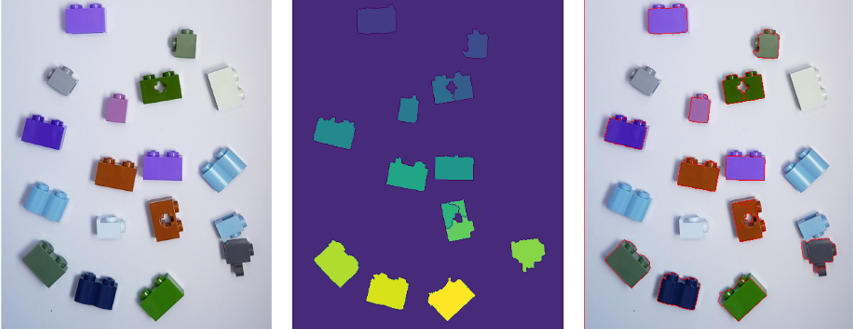
\includegraphics[width=0.8\textwidth]{images/trait_image.png}
\end{center}

\vfill

\textit{Ce sujet est disponible au format électronique sur le site du LEnsE - https://lense.institutoptique.fr/ dans la rubrique Année / Première Année / Interfaçage Numérique S6 / Bloc Images et OpenCV.}


% Bottom of the page
%{\textbf{\large {Année universitaire} 2024-2025}}

\end{center}
\end{titlepage}

\newpage
\strut % empty page

\newpage
\pagestyle{empty}

\begin{minipage}[c]{.25\linewidth}
	
\includegraphics[width=5cm]{images/Logo-LEnsE.png}
\end{minipage} \hfill
\begin{minipage}[c]{.4\linewidth}

\begin{center}
\vspace{0.3cm}
{\Large \textsc{Interfaçage Numérique}}

\medskip

6N-047-SCI \qquad \textbf{\large Bloc Images/OpenCV}

\end{center}
\end{minipage}\hfill

\vspace{0.5cm}

\noindent \rule{\linewidth}{1pt}

{\noindent\Large  \rule[-7pt]{0pt}{30pt} \textbf{Images et OpenCV}}

\noindent \rule{\linewidth}{1pt}

\bigskip 

%%%%%%%%%%%%%%%%%%%%%%%%%%%%%%%%%%%%%%%%%%%%%%%%
%%%%%%%%%%%%%    A A V

{\large À l'issue des séances de TP concernant le \textbf{bloc de traitement d'images avec OpenCV}, les étudiant$\cdot$es seront capables d'utiliser OpenCV pour manipuler des images et appliquer des traitements simples : erosion/dilatation, filtres de lissage, masques...}

\medskip

%%%%%%%%%%%%%%%%%%%%%%%%%%%%%%%%%%%%%%%%%%%%%%%%
%%%%%%%%%%%%%    Ressources

\section{Ressources}

Un tutoriel sur les bases d'OpenCV est disponible à l’adresse suivante : 

\href{https://iogs-lense-training.github.io/image-processing/}{https://iogs-lense-training.github.io/image-processing/}

Un \textbf{kit d'images} est disponible sur le site du LEnsE dans la rubrique \textit{Année / Première Année / Interfaçage Numérique S6 / Bloc Images et OpenCV / Kit d'images}. 

Des \textbf{fichiers de fonctions} sont disponibles sur le site du LEnsE dans la rubrique\textit{Année / Première Année / Interfaçage Numérique S6 / Bloc Images et OpenCV / Répertoire vers codes à tester}. 


Quelques exemples et explications sur les différents pré-traitements d'images est disponible sur le site du LEnsE dans la rubrique \textit{Année / Première Année / Interfaçage Numérique S6 / Bloc Images et OpenCV / Image Processing with OpenCV}. 

%%%%%%%%%%%%%%%%%%%%%%%%%%%%%%%%%%%%%%%%%%%%%%%%
%%%%%%%%%%%%%    Déroulement

\section{Déroulement du bloc}

\begin{description}
	\item[Etape 0 - 30 min] Ouvrir une image et faire son histogramme
	\item[Etape 1 - 30 min] Couleur vers niveau de gris
	\item[Etape 2 - 30 min] Seuillage et binarisation d'une image
	\item[Etape 3 - 60 min] Erosion, Dilatation et Gradient
	\item[Etape 4 - 90 min] Lissage du bruit
	\item[Etape 5 - 90 min] Isoler des éléments verticaux (ou horizontaux) dans une image grâce à des opérateurs morphologiques spécifiques
	\item[Etape 6 - 90 min] Détecter des contours et des points d'intérêt
	\item[Etape 7 - 90 min] Segmenter une image par la méthode de Watershed
	
\end{description}
	
	

\newpage
\section{Primitives}

En traitement d'image, les \textbf{primitives} sont les éléments fondamentaux ou les structures de base qui composent une image, sur lesquels des algorithmes peuvent opérer pour effectuer des analyses ou des traitements. 

Les primitives servent de \textbf{points de départ} pour la reconnaissance d'objets, l'analyse de scène, la segmentation d'image ou la reconstruction 3D. Par exemple, pour détecter un visage dans une image, l'algorithme peut commencer par identifier des primitives simples comme les yeux (points ou régions sombres), puis les relier pour former une structure cohérente.

\bigskip

On peut distinguer 3 catégories de primitives.

\subsection{Primitives de bas niveau}

Ce sont les entités les plus simples extraites directement des pixels de l'image. 

Par exemple :

\begin{itemize}
	\item Points : des pixels isolés ou des points d'intérêt
	\item Lignes ou segments : des ensembles de pixels alignés détectés par des algorithmes de détection de bord
	\item Contours : les frontières des objets définis par des changements d'intensité ou de couleur
	\item Régions : des groupes de pixels connectés ayant des propriétés similaires.
\end{itemize}


\subsection{Primitives de niveau intermédiaire}

Ces primitives sont obtenues en combinant ou en analysant les primitives de bas niveau. 

Par exemple :

\begin{itemize}
	\item Formes géométriques : rectangles, cercles, polygones
	\item Lignes ou segments : des ensembles de pixels alignés détectés par des algorithmes de détection de bord
	\item Objets simples : identification d'objets à partir de leurs contours ou formes.
\end{itemize}

\subsection{Primitives de haut niveau}

Ces primitives sont plus abstraites et dépendent de la compréhension sémantique de l'image. 

Par exemple :

\begin{itemize}
	\item Objets complexes : reconnaissance d'éléments comme des personnes ou des animaux
	\item Relations spatiales : liens entre différents objets (par exemple, un objet en avant d'un autre).
\end{itemize}




\newpage
%%%%%%%%%%%%%    Etape 0
\section{Ouvrir une image sous OpenCV et afficher son histogramme}

\begin{center} \textbf{\textit{Temps conseillé : 30 min}} \end{center}

\begin{mdframed}[style=sidebar,frametitle={}]
Notions : \href{https://iogs-lense-training.github.io/image-processing/contents/opencv.html#open-an-image
}{\textit{Open an image}} - \href{https://iogs-lense-training.github.io/image-processing/contents/opencv.html#display-an-image
}{\textit{Display an image}} - \href{https://iogs-lense-training.github.io/image-processing/contents/opencv.html#enhance-the-image-contrast-and-brightness}{\textit{Calculate the histogram}}
\end{mdframed}
 
\Manip Créer un nouveau projet sous PyCharm et impoter la bibliothèque OpenCV2.

\Manip Ouvrir l'image \textsl{robot.jpg} du kit d'images fourni, en niveau de gris. Afficher l'image.

\Quest Quelle est la taille de l'image ? Quel est le type d'un élément ?

\Manip Calculer l'histogramme de l'image et l'afficher.

\medskip

\textit{Il peut être intéressant de \textbf{créer une fonction qui affiche automatiquement l'histogramme} d'une image à partir de ses données. Elle sera très utile dans la suite du TP pour voir l'impact des effets appliqués sur les images.}


%%%%%%%%%%%%%    Etape 1
\section{Couleur vers niveau de gris}

\begin{center} \textbf{\textit{Temps conseillé : 30 min}} \end{center}

Voir l'impact de la loi de transformation de RGB vers Gray.


%%%%%%%%%%%%%    Etape 2
\section{Seuillage et binarisation}

\begin{center} \textbf{\textit{Temps conseillé : 30 min}} \end{center}




%%%%%%%%%%%%%    Etape 3
\section{Erosion, dilatation et gradient}

\begin{center} \textbf{\textit{Temps conseillé : 60 min}} \end{center}

On se propose ici d'analyser l'impact de différents procédés de pré-traitements (érosion, dilatation et gradient) sur une image.

\medskip

Les pré-traitements à étudier sont à réaliser sur l'image \textsl{a\_letter\_noise.jpg} du kit d'images fourni. Vous pourrez utiliser la fonction \textsl{zoom\_array()} fournie dans le fichier \textsl{images\_manipulation.py} afin d'augmenter la taille des images à analyser. 

\medskip

Pour faciliter l'analyse des images, on propose le code suivant permettant d'afficher 3 images en parallèle sur un même graphique :

\begin{lstlisting}
fig, ax = plt.subplots(nrows=1, ncols=3)    
ax[0].imshow(image_data_1, cmap='gray')
ax[0].set_title('Title Image 1')  
ax[1].imshow(image_data_2, cmap='gray')
ax[1].set_title('Title Image 2')
ax[2].imshow(image_data_3, cmap='gray')
ax[2].set_title('Title Image 3')
\end{lstlisting}


\subsection{Opérations de pré-traitement}

Les opérations de pré-traitement dans le traitement d'images sont essentielles pour \textbf{améliorer la qualité des images} avant d'appliquer des algorithmes plus complexes, comme la segmentation, la détection d'objets ou la classification. Ces étapes de pré-traitement visent à \textbf{réduire le bruit} ou \textbf{améliorer la structure de l'image}. 

Parmi les opérations de pré-traitement classiques, on peut citer :

\begin{itemize}
	\item \textbf{Correction des couleurs} : Balance des blancs, Correction gamma, Amélioration de contraste...
	\item \textbf{Réduction de bruit} : Filtrage linéaire pour atténuer les bruits sans trop affecter les détails importants de l'image, Filtrage non linéaire pour éliminer les bruits impulsionnels, Filtrage anisotrope...
	\item \textbf{Opérations morphologiques} : érosion pour éliminer du bruit, dilatation pour combler des lacunes dans les objets, ouverture et fermeture pour enlever les petites anomalies ou remplir les petits trous dans une image
	\item \textbf{Filtrage fréquentiel} pour éliminer ou atténuer des fréquences particulières (comme des motifs de bruit répétitifs) 
\end{itemize}

\subsection{Eléments structurants d'une convolution (noyau)}

\begin{mdframed}[style=sidebar,frametitle={}]
Notions : \href{https://iogs-lense-training.github.io/image-processing/contents/opencv_erod_dila.html#kernels-for-erosion-and-dilation}{\textit{Structuring Elements (kernels)}} 
\end{mdframed}

Les \textbf{transformations dites morphologiques} se basent sur l'application d'un \textbf{élément structurant} (ou noyau) que l'on va superposer sur chaque pixel de l'image. 

\Manip Générer un noyau en forme de croix de taille 3 par 3 pixels et afficher ce noyau.

\Quest Quel est le type de l'objet noyau résultant ?

\Manip Générer un second noyau en forme de carré de taille 3 par 3 pixels et afficher ce noyau.

\newpage
\subsection{Opérations d'érosion et de dilatation}

\begin{mdframed}[style=sidebar,frametitle={}]
Notions : \href{https://iogs-lense-training.github.io/image-processing/contents/opencv_erod_dila.html#erosion-operation}{\textit{Erosion}} - \href{https://iogs-lense-training.github.io/image-processing/contents/opencv_erod_dila.html#dilation-operation}{\textit{Dilation}} 
\end{mdframed}

\Manip Appliquer une opération d'érosion sur l'image \textsl{a\_letter\_noise.jpg} avec, indépendamment, les deux noyaux précédemment générés. 

\Manip Afficher les deux images ainsi que l'image originale sur un même graphique pour les comparer.

\Manip De la même manière, utiliser une opération de dilatation sur cette même image à l'aide des deux noyaux précédemment générés. Afficher également un comparatif des images résultantes.

\Quest Que pouvez-vous conclure sur l'utilité des opérations d'érosion et de dilatation sur une image ?

\subsection{Opérations d'ouverture et de fermeture}

\begin{mdframed}[style=sidebar,frametitle={}]
Notions : \href{https://iogs-lense-training.github.io/image-processing/contents/opencv_open_close.html#opening-operation}{\textit{Opening}} - \href{https://iogs-lense-training.github.io/image-processing/contents/opencv_open_close.html#closing-operation}{\textit{Closing}} 
\end{mdframed}

\Manip Appliquer une opération d'ouverture (\textit{opening}) sur l'image \textsl{a\_letter\_noise.jpg} avec, indépendamment, les deux noyaux précédemment générés. 

\Manip Afficher les deux images ainsi que l'image originale sur un même graphique pour les comparer.

\Manip De la même manière, utiliser une opération de fermeture sur cette même image à l'aide des deux noyaux précédemment générés. Afficher également un comparatif des images résultantes.

\Quest Que pouvez-vous conclure sur l'utilité des opérations d'ouverture et de fermeture sur une image ?

% L'opération d'opening est utile pour supprimer les petits bruits tout en maintenant la forme et la taille des objets plus grands dans l'image.


\subsection{Opération de gradient}

Une autre opération, appelée \textbf{gradient}, calcule la différence entre une dilatation et une érosion sur une même image. 

Il est possible de la mettre en pratique à l'aide de l'instruction suivante :

\begin{lstlisting}
gradient_image = cv2.morphologyEx(image, cv2.MORPH_GRADIENT, kernel)
\end{lstlisting}

\Manip Appliquer une opération de gradient sur l'image \textsl{robot.jpg} avec, indépendamment, les deux noyaux précédemment générés. 

\Manip Afficher les deux images ainsi que l'image originale sur un même graphique pour les comparer.

\Quest Que pouvez-vous conclure sur l'utilité de l'opération de gradient sur une image ?

% Le gradient met en évidence les bords des objets dans une image, ce qui peut être utile pour détecter des contours ou des transitions nettes dans l'intensité des pixels.


%%%%%%%%%%%%%    Etape 4
\section{Lissage du bruit}

\begin{center} \textbf{\textit{Temps conseillé : 90 min}} \end{center}

\subsection{Générer du bruit sur des images}

\begin{mdframed}[style=sidebar,frametitle={}]
Notions : \href{https://iogs-lense-training.github.io/image-processing/contents/opencv.html#histogram-of-an-image}{\textit{Histogram of an image}} 
\end{mdframed}

On se propose d'étudier la fonction \textsl{generate\_gaussian\_noise\_image()} fournie dans le fichier \textsl{images\_manipulation.py}.

\Manip Tester l'exemple fourni dans le fichier \textsl{noise\_test1.py}.

\Quest Comment vérifier la distribution du bruit généré par cette fonction ?

\medskip

On se propose d'étudier la fonction \textsl{generate\_uniform\_noise\_image()} fournie dans le fichier \textsl{images\_manipulation.py}.

\Manip Tester l'exemple fourni dans le fichier \textsl{noise\_test2.py}.

\Quest La distribution du bruit généré par cette fonction est-elle uniforme ?

\Manip A l'aide de la fonction \textsl{generate\_gaussian\_noise\_image\_percent()}, générer un bruit gaussien de moyenne 30 et d'écart-type 20 sur 10\% de l'image \textsl{robot.jpg} ouverte précédemment en nuance de gris. Visualiser le résultat.



\newpage
\subsection{Comparer différents filtres de lissage}

On se propose à présent d'analyser l'impact de différents filtres de lissage  (flou gaussien, filtre médian et filtre moyenneur) sur une image.

Pour ces trois types de filtres, répéter les étapes suivantes :

\Manip Appliquer une opération de lissage avec le filtre souhaité sur l'image \textsl{robot.jpg} avec un noyau de 15 x 15 pixels.

\Manip Stocker dans une matrice la différence entre l'image originale et l'image lissée.

\Manip Afficher l'image originale, l'image lissée et la différence de deux images sur un même graphique pour les comparer.

\Manip Ajouter du bruit gaussien sur l'image et appliquer à nouveau le filtre gaussien. Afficher l'image originale, l'image lissée et la différence de deux images sur un même graphique pour les comparer.

\Quest Que pouvez-vous conclure sur l'utilité d'un tel filtre ?

\textit{Vous pourrez également regarder l'impact de la taille du noyau sur l'image lissée finale.}


\subsubsection{Filtre de type gaussien}

\Manip Appliquer une opération de lissage de type \textsc{Gaussian Blur} sur l'image \textsl{robot.jpg} avec un noyau de 15 x 15 pixels (\textsl{cv2.GaussianBlur}).

\subsubsection{Filtre de type médian}

\Manip Appliquer une opération de lissage de type \textsc{Median Blur} sur l'image \textsl{robot.jpg} avec un noyau de 15 x 15 pixels (\textsl{cv2.medianBlur}).

\subsubsection{Filtre de type moyenneur (mean ou box)}

\Manip Appliquer une opération de lissage de type \textsc{Averaging Blur} sur l'image \textsl{robot.jpg} avec un noyau de 15 x 15 pixels (\textsl{cv2.blur}).


\newpage	
%%%%%%%%%%%%%    Etape 5
\section{Isoler des éléments d'une image grâce à des opérations linéaires}

\begin{center} \textbf{\textit{Temps conseillé : 90 min}} \end{center}

Les opérateurs d'érosion et de dilatation permettent d'extraire des informations particulières dans l'image à partir du moment où les éléments structurants (noyaux de convolution) sont judicieusement choisis.

On va chercher ici à détecter les lignes horizontales et verticales de l'image \textsl{\textit{forms\_opening\_closing.png}} :

\begin{center}
	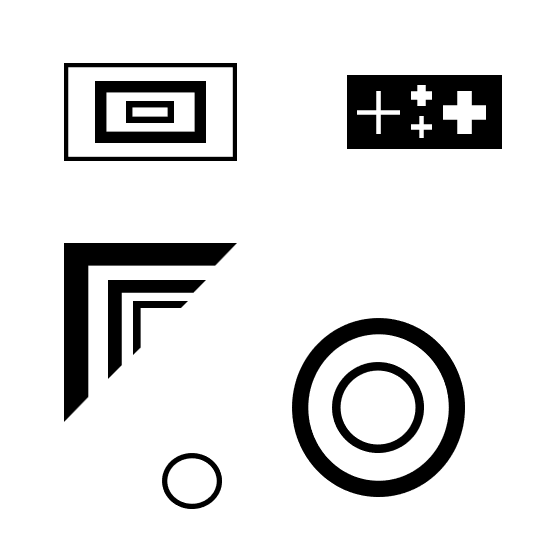
\includegraphics[width=0.4\textwidth]{images/forms_opening_closing_inv.png}
\end{center}


\Manip Tester l'exemple fourni dans le fichier \textsl{line\_detection.py}.

\Manip Afficher les images aux différentes étapes du traitement.

\Quest Analyser les différentes phases du traitement. Quelle est la forme du noyau utilisé ? Quel est l'impact de sa taille sur les éléments détectés ?

\Manip A partir de l'exemple précédent, écrire un script qui permet de détecter les lignes verticales de cette image et afficher le résultat.

\Manip Tester ces deux exemples sur d'autres images.




%%%%%%%%%%%%%    Etape 6
\section{Détecter des contours et des points d'intérêt}

Canny et Harrys

\begin{center} \textbf{\textit{Temps conseillé : 90 min}} \end{center}



%%%%%%%%%%%%%    Etape 7
\section{Segmenter une image par la méthode de Watershed}

Watershed

\begin{center} \textbf{\textit{Temps conseillé : 90 min}} \end{center}

%%%%%%%%%%%%%%%%%%%%%%%%%%%%%%%%%%%%%%%%%%%%%%%%
%%% RESSOURCES COMPLEMENTAIRES		

\newpage
\begin{center}
	\begin{minipage}{2.5cm}
	\begin{center}
		
\includegraphics[width=5cm]{images/Logo-LEnsE.png}
	\end{center}
\end{minipage}\hfill
\begin{minipage}{10cm}
	\begin{center}
	\textbf{Institut d'Optique Graduate School }\\[0.1cm]
    \textbf{Interfaçage Numérique}


	\end{center}
\end{minipage}\hfill


\vspace{2cm}


{\Large \bfseries \textsc{Interfaçage Numérique}} \\[0.5cm]
{\large \bfseries Travaux Pratiques} \\[0.2cm]
Semestre 6

\vspace{1cm}

% Title
\rule{\linewidth}{0.4mm} \\[0.4cm]
{ \Large \bfseries\color{violet_iogs} Ressources \\[0.4cm] }
\rule{\linewidth}{0.4mm} \\[1cm]
{\large Bloc Images et OpenCV}

\end{center}

\vspace{3cm}

\textbf{\large Liste des ressources}
\begin{itemize}
	\item \hyperref[doc:image_proc]{Image Processing / Key concepts}
\end{itemize}

\vfill

\newpage
\strut % empty page


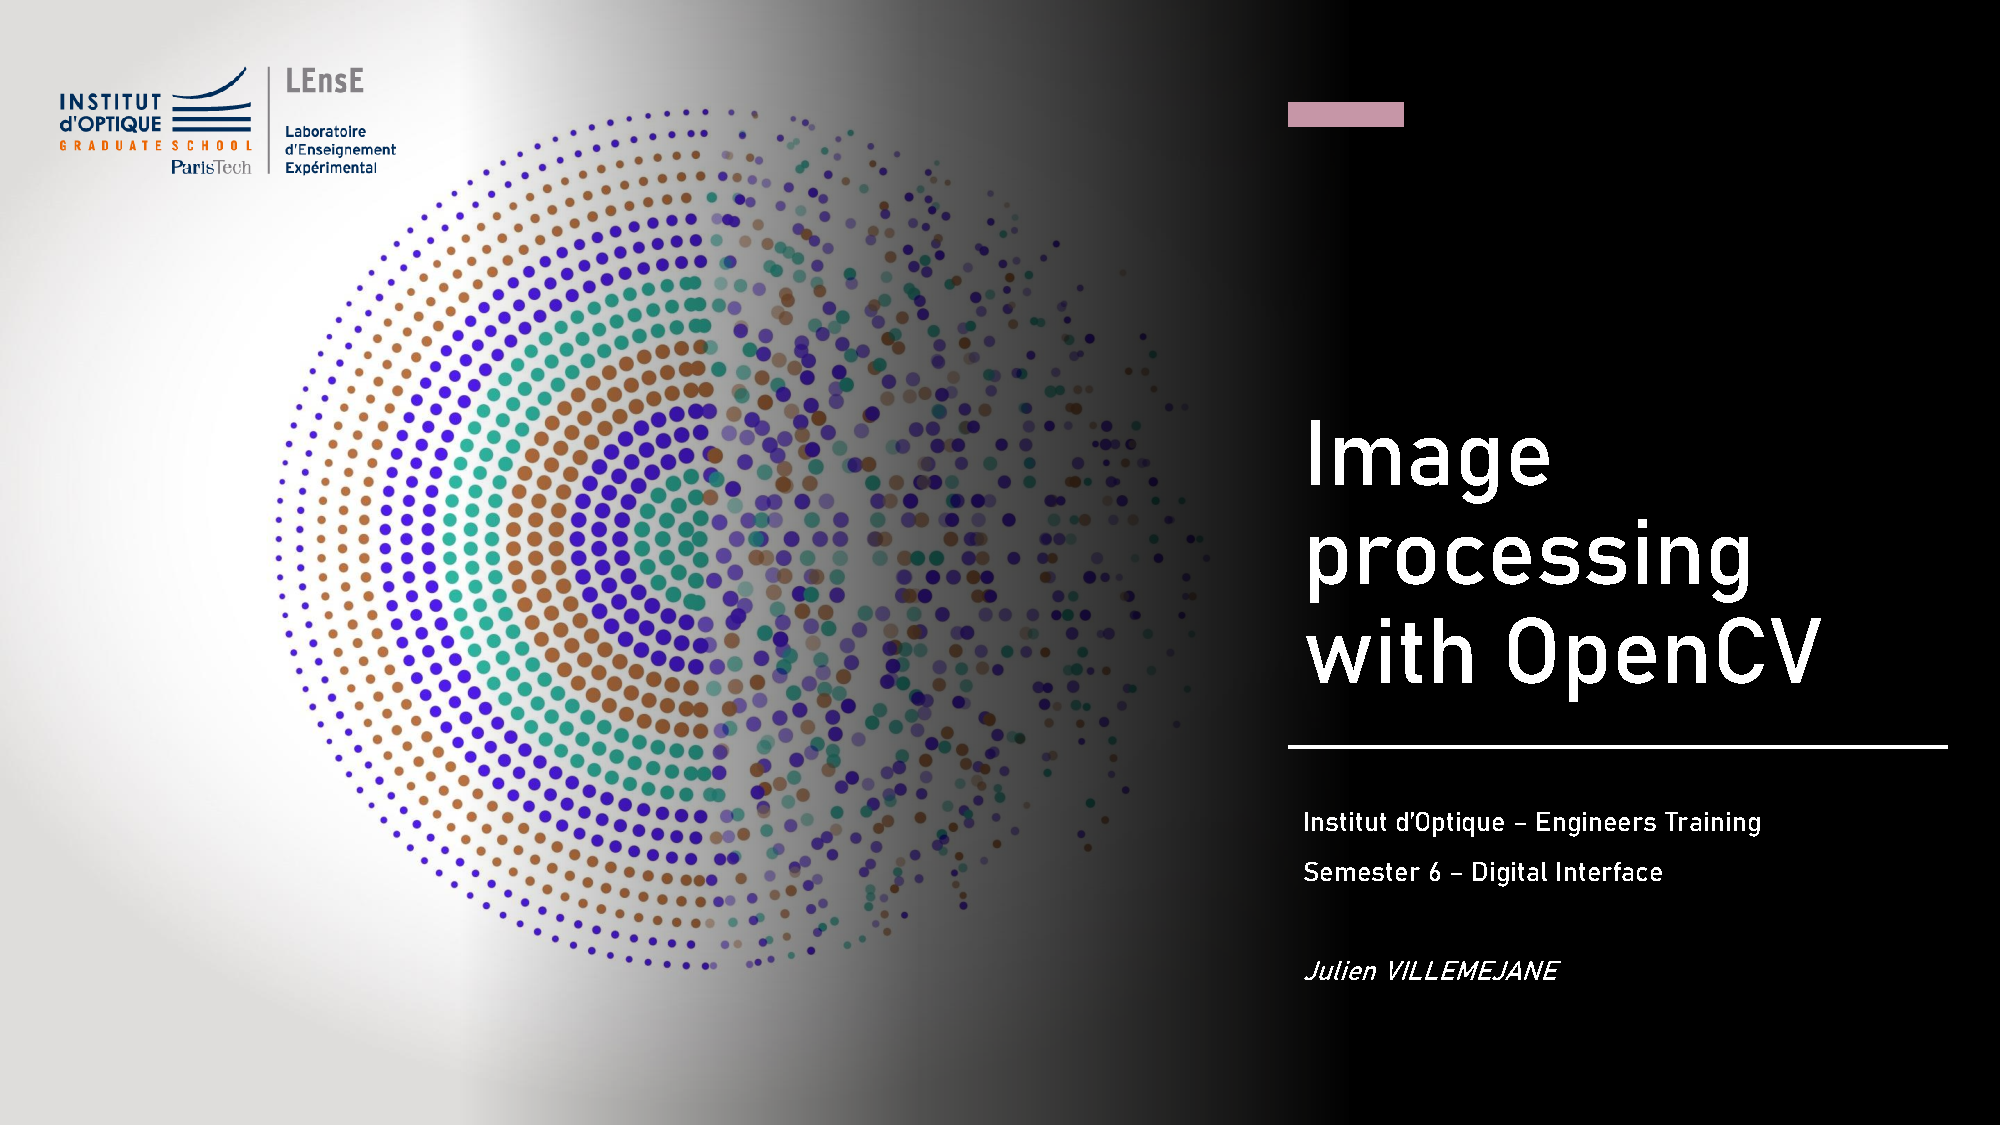
\includepdf[pages={1,4}, nup=1x2, pagecommand={\section{\texorpdfstring{\hspace{-1em}}{Image Processing}}}\label{doc:image_proc}]{../docs/Image_Processing.pdf}
\includepdf[pages={5,8,12,14,16,17,18,20,21,22,23,24,25,31}, nup=1x2]{../docs/Image_Processing.pdf}

\end{document}


